\chapter{Step 01: Logic Gates}
\label{ch:step01}

Our first design has no state at all: two buttons, two LEDs, and a few gates in
between. This is little hardware, but enough to meet the basic parts of
SystemVerilog, to follow the design through all the tools of
Figure~\ref{fig:toolflow}, and to simulate it. Everything is in the directory
\cc{01_logic_gates}.

\section{The Circuit}
\label{sec:step01-circuit}

Call the two buttons $a$ and $b$ (pressed means 1) and the two LEDs
$\mathit{out}_1$ and $\mathit{out}_2$ (1 means on). The circuit computes
\[
  \mathit{out}_1 = (a \wedge b) \vee a, \qquad
  \mathit{out}_2 = a \vee b .
\]
You would draw it in CircuitVerse as in Figure~\ref{fig:step01-netlist}: an AND
gate and two OR gates. In fact, this figure was not drawn by hand: it was
generated from the SystemVerilog description by \cc{make png}, which we come
back to in Section~\ref{sec:step01-pictures}.

\begin{figure}[ht]
\centering
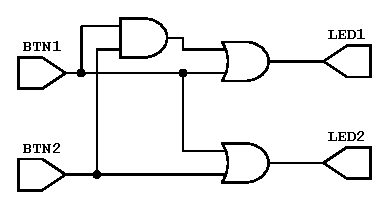
\includegraphics[width=0.62\linewidth]{figures/01_netlist.pdf}
\caption{The circuit of step 01, as drawn by \cc{make svg} from \cc{test.sv}.
The pins on the left and right are the ports of the module.}
\label{fig:step01-netlist}
\end{figure}

\section{The Description in SystemVerilog}
\label{sec:step01-sv}

This is the complete description:

\svfile{01_logic_gates/test.sv}

Read it as a description of the circuit in Figure~\ref{fig:step01-netlist},
piece by piece.

\textbf{A module is a box with pins.} Everything between \cc{module} and
\cc{endmodule} describes one circuit, here called \cc{test}. The list in
parentheses are its \term{ports}: the wires that leave the box, each one an
\cc{input} or an \cc{output}. In CircuitVerse terms, a module is what you get
when you turn a circuit into a subcircuit, and the ports are its inputs and
outputs.

Because \cc{test} is the outermost module, the \term{top module}, its ports
are the pins of the chip. Their names are not arbitrary: \cc{BTN1}, \cc{BTN2},
\cc{LED1} and \cc{LED2} are names from \cc{icebreaker.pcf}
(Section~\ref{sec:board}), and that is how nextpnr knows which pin of the FPGA
each port is.

\textbf{\cc{logic} declares a signal.} The line \cc{logic a, b;} declares two
wires inside the box, each carrying one bit. The type \cc{logic} says only
that the signal carries a logic value; whether it ends up as a plain wire or as
the output of a flip-flop follows from how we use it, as we see in the next
chapter.

\textbf{\cc{assign} connects.} \cc{assign a = BTN1;} says that the wire
\cc{a} is permanently connected to the input \cc{BTN1}. It is not an
assignment in the sense of a programming language, which happens once when the
line is executed. It is a statement about the circuit that holds all the time:
whatever value \cc{BTN1} has, \cc{a} has it too. The four \cc{assign}
statements only give the pins more convenient names. This separates the logic
of our design (\cc{a}, \cc{b}, \cc{out1}, \cc{out2}) from the question which
pin is which, and we can change one without the other.

\textbf{\cc{always_comb} describes combinational logic.} The block
\begin{lstlisting}
always_comb begin
    out1 = a & b | a;
    out2 = a | b;
end
\end{lstlisting}
says: \cc{out1} and \cc{out2} are computed from the signals on the right-hand
sides, by a circuit without memory. Whenever an input changes, the outputs
follow. The operators are the Boolean operations you know:
\begin{center}
\begin{tabular}{cccl}
\toprule
SystemVerilog & logic & name & \\
\midrule
\cc{&} & $\wedge$ & AND & \\
\cc{|} & $\vee$ & OR & \\
\cc{^} & $\xor$ & XOR & (exclusive or) \\
\cc{~} & $\neg$ & NOT & \\
\bottomrule
\end{tabular}
\end{center}
As in arithmetic, where $\cdot$ binds stronger than $+$, \cc{&} binds stronger
than \cc{|}, so \cc{a & b | a} means \cc{(a & b) | a}.

Here the two statements in the block are independent, so their order does not
matter at all. We could also have written \cc{assign out1 = a & b | a;}, which
describes the same circuit. \cc{always_comb} becomes useful when the logic
needs case distinctions, which we see in later steps.

\begin{pitfall}
SystemVerilog looks like a programming language, and the \cc{=} in
\cc{always_comb} looks like an assignment that is executed at some point. It is
not. The whole module describes a circuit that exists all the time, and all of
its parts work in parallel. There is no ``first line'' that runs before the
second, just as there is no first gate in Figure~\ref{fig:step01-netlist}.
\end{pitfall}

\begin{exercise}
\label{ex:step01-absorb}
Simplify $(a \wedge b) \vee a$. What does that mean for \cc{LED1}?
\end{exercise}

\section{From test.sv to the Chip}
\label{sec:step01-synth}

In the directory \cc{01_logic_gates}, the command \cc{make synth} runs the
tools of Figure~\ref{fig:toolflow} up to the bitstream. It prints the
commands it runs:

\outputfile{step01_make_synth.txt}

Before that, \cc{make} has called \cc{sv2v} to produce \cc{test.v}:

\outputfile{step01_make_v.txt}

The option \cc{--define=SYNTHESIS} matters only from step 08 on: there, parts
of a file are meant for simulation only, and \cc{SYNTHESIS} switches them off.

\subsection*{What yosys makes of it}
\label{sec:step01-yosys}

yosys writes its report to \cc{test.log}. The interesting part is at the end, a
list of the building blocks of the netlist:

\outputfile{step01_yosys_stat.txt}

Four ports, six wires, and exactly \emph{one} building block, an
\cc{SB_LUT4}: one lookup table with four inputs. Three gates became a single
LUT, and \cc{LED1} needs no logic at all. If you solved
Exercise~\ref{ex:step01-absorb}, you know why: $(a \wedge b) \vee a = a$, so
\cc{LED1} is simply connected to \cc{BTN1}, and yosys found that out by itself.
\cc{LED2} needs a LUT for $a \vee b$.

Which LUT? The netlist \cc{test.json} contains, for every building block, its
type and its parameters. For our LUT:

\outputfile{step01_lut.txt}

\cc{LUT_INIT} are the 16 configuration bits of Section~\ref{sec:lut}, written
from $t_{15}$ on the left down to $t_0$ on the right. The netlist also says
how the LUT is connected: \cc{BTN1} drives input $x_3$, \cc{BTN2} drives $x_2$,
and the inputs $x_1$ and $x_0$ are fixed to 0. So the LUT selects the bit
\[
  t_{8\cdot\mathtt{BTN1} + 4\cdot\mathtt{BTN2}} ,
\]
which is $t_0 = 0$ if no button is pressed, and $t_4 = t_8 = t_{12} = 1$ if at
least one is. That is $\mathtt{BTN1} \vee \mathtt{BTN2}$, exactly as it should
be. The other twelve bits are never selected; yosys sets them to 1, but any
value would do.

\subsection*{What nextpnr makes of it}

nextpnr places the LUT on one of the 5280 logic cells, connects the four pins,
and reports what it used:

\outputfile{step01_pnr_util.txt}

\cc{ICESTORM_LC} are the logic cells, \cc{SB_IO} the I/O pins. Three logic
cells for one LUT? The other two produce the constants 0 and 1, which the
unused LUT inputs are connected to. (Our report from
Appendix~\ref{app:tools}, \cc{make report}, shows the same numbers.)

nextpnr also computes how long a signal takes from an input pin to an output
pin. For the slowest path, from \cc{BTN2} to \cc{LED2}:

\outputfile{step01_pnr_path.txt}

The numbers in parentheses are positions on the chip: the pin of \cc{BTN2}
at the lower edge, the LUT in the middle, the pin of \cc{LED2} at the upper
edge. The LUT itself takes 1.21\,ns, and the wires to and from it take 9.77\,ns.
This is typical for FPGAs: the routing is usually slower than the logic. For
us it does not matter here, since nobody presses buttons within 11\,ns. Once a
clock is involved, it will.

\subsection*{Programming the board}

\cc{make prog} does everything \cc{make synth} does and then calls
\cc{iceprog test.bin}, which writes the bitstream into the flash of the board
and restarts the FPGA. A second later, the LEDs follow the buttons: \cc{LED1}
is on while the first button is pressed, \cc{LED2} while one of the two is
pressed.

\begin{exercise}
\label{ex:step01-xor}
Replace \cc{out2 = a | b;} by \cc{out2 = a ^ b;}. Predict the value of
\cc{LUT_INIT} for the LUT of \cc{LED2}, then check it with \cc{make test.json}
and a look into \cc{test.json}.
\end{exercise}

\section{Simulation}
\label{sec:step01-sim}

Programming the board is the final test, but it is a poor tool for finding
mistakes: you see only what reaches a pin. In a \term{simulation}, a program
computes how all signals of the design change over time, and we can look at
every one of them.

We use Verilator. It translates the design into a C++ class \cc{Vtest}, whose
member variables are the ports of the module. A small C++ program, the
\term{testbench} \cc{tb_test.cpp}, creates such an object, sets its inputs and
calls \cc{eval()}, which computes the outputs. Here is its main loop:

\cpppart{firstline=21,lastline=45}{01_logic_gates/tb_test.cpp}

The variable \cc{sim_time} counts steps of the simulation; it has no unit, it is
just an index. At time 5 the testbench presses the first button, at time 8
both, at time 11 the second, and at all other times none. After each
\cc{eval()}, \cc{m_trace->dump(sim_time)} records the values of all signals in
the file \cc{waveform.vcd}, a \term{value change dump}.

\cc{make sim} (or just \cc{make}) calls Verilator, compiles the generated C++
code together with the testbench, and runs the result:

\outputfile{step01_make_sim.txt}

The simulation itself prints nothing. Its result is \cc{waveform.vcd}, and
\cc{make surfer} (or \cc{make waves} for GTKWave) shows it in a waveform
viewer. Figure~\ref{fig:step01-waves} shows what you see.

\begin{figure}[ht]
\centering
\begin{tikzpicture}[x=6.5mm,y=5mm]
  \foreach \name/\y in {BTN1/6, BTN2/4.5, LED1/3, LED2/1.5} {
    \node[anchor=east,font=\small\ttfamily] at (-0.3,\y+0.3) {\name};
    \draw[black!15] (0,\y) -- (15,\y);
  }
  % BTN1 high on [5,6) and [8,9)
  \draw[signal] (0,6) -- (5,6) -- (5,6.6) -- (6,6.6) -- (6,6) -- (8,6) -- (8,6.6) -- (9,6.6) -- (9,6) -- (15,6);
  % BTN2 high on [8,9) and [11,12)
  \draw[signal] (0,4.5) -- (8,4.5) -- (8,5.1) -- (9,5.1) -- (9,4.5) -- (11,4.5) -- (11,5.1) -- (12,5.1) -- (12,4.5) -- (15,4.5);
  % LED1 = BTN1
  \draw[signal,draw=green!45!black] (0,3) -- (5,3) -- (5,3.6) -- (6,3.6) -- (6,3) -- (8,3) -- (8,3.6) -- (9,3.6) -- (9,3) -- (15,3);
  % LED2 = BTN1 | BTN2
  \draw[signal,draw=green!45!black] (0,1.5) -- (5,1.5) -- (5,2.1) -- (6,2.1) -- (6,1.5) -- (8,1.5) -- (8,2.1) -- (9,2.1) -- (9,1.5) -- (11,1.5) -- (11,2.1) -- (12,2.1) -- (12,1.5) -- (15,1.5);
  \foreach \t in {0,5,8,11,15} {
    \draw[black!40] (\t,0.9) -- (\t,0.7) node[below,font=\scriptsize] {\t};
  }
  \node[note,anchor=west] at (15.3,0.4) {\cc{sim_time}};
\end{tikzpicture}
\caption{The waveforms of step 01: the inputs set by the testbench, and the
outputs computed by the simulation.}
\label{fig:step01-waves}
\end{figure}

In this design, the outputs follow the inputs within the same step. That is
what combinational means, and in the simulation there are no wires that take
time. The simulation shows the logic, not the 11\,ns of the real chip.

\begin{exercise}
\label{ex:step01-tb}
Change the testbench so that it also presses only the second button for a
while, and check in the waveform viewer that \cc{LED1} stays off and \cc{LED2}
goes on.
\end{exercise}

\section{Pictures of a Design}
\label{sec:step01-pictures}

\cc{make svg} and \cc{make png} produce pictures like
Figure~\ref{fig:step01-netlist}. They run yosys with only light processing
(\cc{prep} instead of \cc{synth_ice40}) and let the tool netlistsvg draw the
result. So the picture shows the logic as we wrote it, with an AND and two ORs,
not the single LUT that ends up on the chip. That is what makes it useful: it is
the most direct check that the text describes the circuit we had in mind.

For small designs this is the best way to see a circuit. For the larger steps
the pictures become too big to read, and we turn to other views: how many
logic cells each part of a design uses (\cc{make report}), and where they end
up on the chip (\cc{make floorplan}). Appendix~\ref{app:tools} describes them.

\solutions

\solution
By absorption, $(a \wedge b) \vee a = a$: if $a = 1$ the right side is 1; if
$a = 0$ both terms are 0. So \cc{LED1} is on exactly when the first button is
pressed, and \cc{LED1} needs no gate at all. yosys finds this, and the netlist
connects \cc{LED1} directly to \cc{BTN1}.

\solution
The LUT selects $t_{8\cdot\mathtt{BTN1} + 4\cdot\mathtt{BTN2}}$, and for
$\mathtt{BTN1} \xor \mathtt{BTN2}$ we need $t_0 = 0$, $t_4 = 1$, $t_8 = 1$,
$t_{12} = 0$. If yosys keeps the inputs as before and again sets the unused
bits like the bit they share the higher inputs with, you get
\cc{0000111111110000}. The unused bits may come out differently; what must
hold is $t_0 = t_{12} = 0$ and $t_4 = t_8 = 1$. (yosys may also connect the
buttons to other inputs of the LUT. Then the positions change, but the rule
for reading them is the same.)

\solution
For example, add a case to the \cc{switch}:
\begin{lstlisting}[language=C++]
case 14:
    dut->BTN1 = 0;
    dut->BTN2 = 1;
    break;
\end{lstlisting}
Since the \cc{default} case releases both buttons again at the next step,
the button is pressed for one step only. To keep it pressed for longer, use a
range of times, for instance with an \cc{if} instead of the \cc{switch}.
